\graphicspath{{chapters/06_discussion/images}}
\chapter{Discussion}

% The Discussion section contains a critical analysis of the results obtained and frames them in the context of the international literature (at least 5, maximum 10 pages).

In this chapter, the results shown in the previous section are discussed, including possible solutions to improve  performance of the package. Some other preliminary results, which were not included due to them being unrelated to the development of the preprocessing section of HiCONA, are also discussed. Again, these analyses were conducted by my tutor, Leonardo Morelli, and are not part of the functionalities implemented by HiCONA; they are though useful for the validation of the performance of HiCONA, or they are exploratory analyses to define what could be implemented into HiCONA. Finally the current state of the package, what is currently available and what could be done in the near future, are all presented.

% PANCALDI SOMEWHERE?

%%%%%%%%%%%%% ABOUT THE ANALYSIS %%%%%%%%%%%%%%%%%%%%%%%

\section{Pixel preprocessing}
In this section, the main steps of the pixel preprocessing procedure are discussed individually. Particular attention is given to the reason why certain choices were made, which are the limitations of these steps and how these steps could be improved upon.

\subsection{Sequencing bias normalization}
One concern that might be raised regarding the preprocessing pipeline adopted by HiCONA is the lack of a sequencing bias normalization step. There are two main reasons for that. First, sequencing biases are expected to affect the pixel counts way less than genomic distance, to the point where it is not unreasonable to assume that the networks obtained with or without sequencing bias normalization should behave almost identically. As mentioned in subsection \ref{par:sequencingbias}, sequencing bias normalization methods assume the bins to be homogeneous in regards to the feature they are normalizing for. This is quite an approximation, considering that even at a 10 kb resolution, which is on the lower end of viable resolutions, the bins are still quite big and heterogeneous, to the point where it is arguable whether the entire normalization actually makes sense or not. These considerations, coupled with the fact that it is unclear which bias normalization algorithms are actually reliable and the fact that integer counts have substantially better properties for computational purposes, led to the choice of not including sequencing bias normalization in the standard package pipeline. Nevertheless, 
HiCONA is fully capable of working with sequencing bias normalized counts, though in a less efficient manner considering it was optimized for non-normalized ones.

\subsection{Genomic distance normalization}
The way HiCONA normalizes for genomic distance was shown to be reliable and consistent, being unstable only at extremely high genomic distances. It must be remarked that, using the current algorithm, if a pixel with high count is the only one for that genomic distance, it is assigned the normalized value of 1. %TODO: Quantify genomic distance
This can reasonably happen only at very high genomic distances, where the number of pixels per genomic distance is very low, and one individual pixel might have a very high count value causing a spike in the expected counts curve. Though it might seem strange to normalize to 1 a pixel with such a high value with respect to its neighboring distances, at genomic distances that high, the actual biological significance of those spikes starts to become debatable, with them being random ligation products or PCR artifacts becoming the more likely option. Losing a few potentially meaningful pixels at these genomic distances does not therefore seem like a major issue. 

In regards to normalization factors computation, it should be noted that, regardless of the usage of \textit{cooltools} or HiCONA, one summary statistic function is computed for each individual chromosome. \textit{Cooltools} does, in fact, go even beyond this, allowing to remove telomeres and centromere, then computing one normalization curve for each arm of the chromosome. The use of one curve per chromosome is to avoid relying on the assumption that random contact probability decays at the same rate in all chromosomes. One might argue that considering all pixels jointly would yield a more robust and less noisy function; while that would indeed be the case, each chromosome has enough pixels to obtain a robust result on its own (aside from chromosome Y due to its significantly smaller size and probably other biological motivations).

\subsection{Pixel filtering}
Pixel filtering led to unexpected results. The step was introduced to both remove pixels which are definitely to be discarded for sparsification to work properly (self-looping and inter-chromosomal ones), as well as to reduce a bit noise and dimensionality prior to sparsification. This last aspect was especially relevant when the tool did not work in chunks and thus table size was still an issue. Though raw counts threshold is probably not needed anymore and was, in fact, not included in the analyses presented, different combinations of genomic distance threshold and normalized counts quantile threshold were tested. Ideally, the distance threshold would be set to the maximal distance for an interaction to be considered biologically relevant, but such threshold has not been clearly defined yet. For the quantile threshold, defining a value is even more complicated, since it is not tied to any biological meaning. It follows that the only real way to choose these parameters is trial and error using educated guesses. 

In terms of filtering itself, the results seem middling; any filtering threshold which provides a significant reduction in pixel number also causes a massive reduction in genomic distance which does not seem to be justifiable prior to network sparsification, making very loose thresholds the only viable option. The need for a filtering step becomes even more debatable when considering that the combination of filtering parameters used does not appear to significantly affect sparsification, if at all. Yet, the choice of filtering parameters affects the consistency of replicates quite a lot, with fold changes which are higher and statistically significant. Further and more systematic testing of parameter combinations could probably lead to even better consistency, though it would be quite demanding in terms of time.

\subsection{Network sparsification}
Regarding network sparsification, a standardized procedure to decide an alpha cutoff was proposed and used throughout all the analyses, removing the need to define arbitrary values, which becomes especially complex when considering that different thresholds are required for different chromosomes. As mentioned, being sparsification scores actual p-values, the usual p-value cutoff of 0.05 seems like a pretty natural choice and it was, in fact, tested as a sparsification score threshold. This value proved far too restrictive with any combination of filtering parameters, to the point where just a couple hundreds of pixels are retained, at most, for each file. This value is therefore not appropriate for this application, and in fact, even the original paper which introduced the algorithm proposed the use of looser thresholds. It must be remarked once more that the objective of this procedure is not to determine the definitely significant pixels themselves, but rather sparsify the network by removing the least significant ones to achieve a network of a manageable size (while still maintaining disconnected components of a reasonable size). 

Both minimal alphas, for a more permissive network, as well as maximal alphas, for a more theoretically robust one, were tested. The choice does not change sparsification results in an appreciable manner, while minimal alphas seem to marginally outperform maximal ones in regards of consistency. For this reason, minimal alphas will probably be the standard option for the package going forward. It must be also stated that the use of minimal alphas seems more appropriate even on a purely theoretical level, since it is more in line with the original network sparsification algorithm in trying not to belittle smaller nodes. 

The aspect which could be considered the big criticality of the sparsification algorithm is how much the median genomic distance is reduced. While it is fair to assume that there are more significant interactions at closer ranges, and thus that sparsification will inevitably reduce median genomic distance, the reduction feels quite heavy. Again, this is not unexpected, considering that the algorithm does not keep genomic distance into account while defining edge importance; one option could be to try and include the distance information in the algorithm, though it seems rather complex and demanding.


\section{Computational performance}

The current implementation of the sparsification algorithm is already quite fast, though many aspects could be tweaked for an even greater speed-up. Regarding integral computation, for instance, the cache of integrals could persist among chunks; this is currently not done since there is a fairly big amount of integrals that are still used only once throughout the entire chromosome sparsification, and keeping all of them in cache needlessly would increase its size drastically. Another option would be to precompute the most common integrals and store them in a tabular file, ready to be loaded as cache when needed. This would lead to a fairly big overhead during the first usage of the package, but could speed-up drastically successive runs. Another aspect which could be optimized are operations on \textit{pandas} dataframes; though vectorized operations are fast, they could be improved by relying on faster structures, such as \textit{polars}\cite{polars2023} dataframes, which work similarly but they are implemented in Rust, making them substantially faster. Dataframe operations could also be sped up using \textit{swifter}\cite{swifter2023}, which allows to split a dataframe in chunks and work in parallel on them. On this topic, it should be mentioned that HiCONA, as of now, does not perform any form of parallelization explicitly, though some operations are implicitly parallelized by \textit{cooler} using \textit{dask}\cite{dask2023}. A pretty substantial speed-up could be obtained by processing the chromosomes in parallel, considering the fact that they are independent from each other. That being said, the library \textit{h5py}\cite{h5py2023}, used to work with \texttt{.hdf5} files and on which \textit{cooler} is based, is implemented with several file locks to prevent corrupting the files while working on them, making parallel writing rather difficult. Overall, considering that the preprocessing times are already quite fast, speeding up these aspects is not currently marked as a top priority.

In terms of RAM usage, the preprocessing was shown to be very efficient, requiring very low amounts of memory. It might be debated that chunk size could be increased, to reduce the number of I/O operations therefore speeding up the procedure while still keeping a relatively low memory footprint. Surprisingly, this is not the case; by increasing chunk size the time per million of pixels to process actually increases. Though no definitive reason was found, this is most likely due to a poor scaling of the \texttt{merge} function of \textit{pandas}, which is used to associate the computed integral values back to the pixels. In any case, a better choice would be to keep the amount of memory of the individual process low, then run multiple of them in parallel on different chromosomes as discussed in the previous paragraph. 

\section{Biological validation}

In the results, biological validation through replicate consistency was analyzed. Overall, the pipeline does not seem to have the highest Jaccard indexes in terms of absolute values, though the sparsification step is very good at retaining the correlation present in the filtered pixels, especially given the right filtering parameters. When considering that the correlation of the filtered files is already very low, it does appear that the issue with low correlation might lie in the biological experiments themselves rather than in the processing pipeline. This would be in line with the fact that the matrix obtained through a single Hi-C experiment is very sparse, therefore requiring multiple experiments to be merged to obtain a denser matrix. The ideal pipeline would be able to increase the correlation among replicates, since this would mean that similar information could be obtained by sequencing less, thus reducing experimental costs. HiCONA does not seem to be at that stage yet.

Another form of biological validation which was performed, but not shown in the results since not strictly tied to the actual implementation, regards functional annotation enrichment. For each bin, it is possible to define which functional element (promoter, enhancer, heterochromatin and others) is the most enriched with respect to the abundance of these functional elements in the genome. Then, it is possible to define the fraction of interactions which occur among any pair of functional elements. By comparing these fractions among different processing steps, such as between total pixels and sparsified pixels, it is possible to define which type of interactions are enriched by the procedure. Ideally, one would like for biologically relevant annotations, such as promoters and enhancers, to be enriched by the step. The annotation enrichment was computed on the individual replicates of IMR90 cells and GM12878 cells at 5 kb resolution, both on the total pixels as well as on the pixels sparsified using distance threshold equal to 100 Mb and quantile threshold equal to 0.01. The annotations used were obtained from the paper of Forcato et al., 2017\cite{toolcomparison2017}, which grouped annotations generated using the tool ChromHMM\cite{chromhmm2014}. For each cell line, the enrichments at each step were averaged, then the $\log_2$ fold change among sparsified and total pixels was determined. This analysis yielded promising results, with a substantial enrichment of promoter, enhancer and zinc finger binding annotations in the sparsified files. This suggests that the sparsification step is able to enrich for pixels which are more likely to be biologically meaningful.

%%%%%%%%%%%%% ABOUT THE PACKAGE %%%%%%%%%%%%%%%%%%%%%%%

\section{Network analysis algorithms}

In HiCONA, a \texttt{HiconaGraph} object is already implemented. Since it inherits from the main \textit{graph-tool} class, it is able to already perform quite a vast set of operations, such as computing network statistics and centrality measures, performing clustering and complex plotting (but the list is much longer). To these functionalities, an \textit{ad hoc} version of node label permutations was added. The algorithm does work properly on mock networks, while it does not seem to work on real Hi-C derived ones. Though this could simply be that there are, in fact, no differences in properties for nodes annotated with different biological functions, this could also be due to how the node annotation is performed. Currently, bins are annotated by intersecting them with a bed-like file and assigning to them the label of any annotation which has any amount of overlap with them. It must be considered though that bins of 5 kb in size are quite big and thus many bins end up being annotated with a lot of labels. This huge overlap of annotations is what could be currently preventing the detection of any significant differences.
% In the animal-community studies field, it has been discussed for a while how node-labels permutation does not actually perform as well as initially though given that most permutations do not satisfy the joint probabilities smth smth dont remember exactly [FIX] \cite{nullmodel2017}; fairly recently, a theoretical proof that node-label permutation perform exactly like non-network-based parametric methods has been published [ADD REFERENCE]. That being said, the network approach INSERT REASON WHY THE NETWORK APPROACH IS STILL GOOD, LIKE INTERPRETABILITY AND SUCH.

Contrast subgraphs extraction is another \textit{ad hoc} analysis algorithm which was planned to be included into HiCONA. Contrast subgraphs extraction is a recently introduced network analysis algorithm for the comparison of networks. Since it has found some success in different biological applications, such as brain network classification as well as comparison of omics data-derived networks\cite{contrast2020, contrast2023}, it seems plausible that it could yield interesting results when applied to the analysis of Hi-C data-derived networks. The algorithm can be roughly summarized as follows. The inputs are two weighted undirected networks defined over the same set of nodes and some tuning parameter $C$. The edge weights are scaled to the range $(0,1]$, then one graph is subtracted edgewise from the other. The heuristic peeling process follows, which is a greedy solution for the densest subgraph problem on networks with negatively weighted edges. Basically, at each step of this iterative procedure, the edge contributing the least to overall graph sum of weights is removed; the parameter $C$ determines how much positive weights are favored with respect to negative ones. In synthesis, the results are one or more contrast subgraphs, which are subgraphs recapitulating the major differences among the two input networks (in a non-symmetric manner). This procedure was tested on sparsified networks obtained using HiCONA, though it does not appear to provide any insightful results. The procedure seems to simply return the difference of the two graphs, and this is likely due to the fact that the sparsified graphs do not have enough overlap. Still, contrast subgraphs might still be considered provided that some major modification of the algorithm is performed.


\section{Package development}

The package was implemented for Python version 3.7 and later, but it should work even for previous versions provided that there is a release of the dependencies for it (though it was not checked since it does not seem particularly relevant). 
The code is styled using \textit{Black}\cite{black2023}, in order for the code formatting to be consistent and compliant with PEP style guidelines\cite{pep2023}. Linting is performed using \textit{Pyflakes}\cite{pyflakes2023}.
All public functions and methods of the package are fully documented and type hinted using the NumPy docstring conventions. For this reason, documentation using \textit{Sphinx}\cite{sphinx2023} is being created and will become the \textit{Read The Docs} page once the package is made available on \textit{PyPI} and \textit{Conda}.
To further support package documentation, \textit{Jupyter}\cite{jupyter2023} notebooks will be created to illustrate standard pipelines. Moreover, now that the package has a partially stable structure, tests are being implemented using \textit{pytest}\cite{pytest2023} to simplify the addition of new features and collaborative work, especially with an open-source model in mind.

As of the time of writing, the code for the preprocessing procedure, therefore the steps from the .cool file to the generation of annotated networks, is almost deployment-ready. Some minor optimizations and refactoring are still required, though no functionality is missing. For what concerns network analysis, the node-labels permutation algorithm is fully implemented and working, though whether it is able to produce meaningful results is still to be verified. Contrast subgraph extraction is currently not included, though it might be in the future if a change in the algorithm or procedure is found to make it work with sparsified networks. Other functionalities will be added overtime when the need for them arises.

In figure \ref{fig:roadmap}, a roadmap summarizing the current state of HiCONA and its future, at least for a few months to come, is presented.

\begin{figure}[ht]
  \centering
  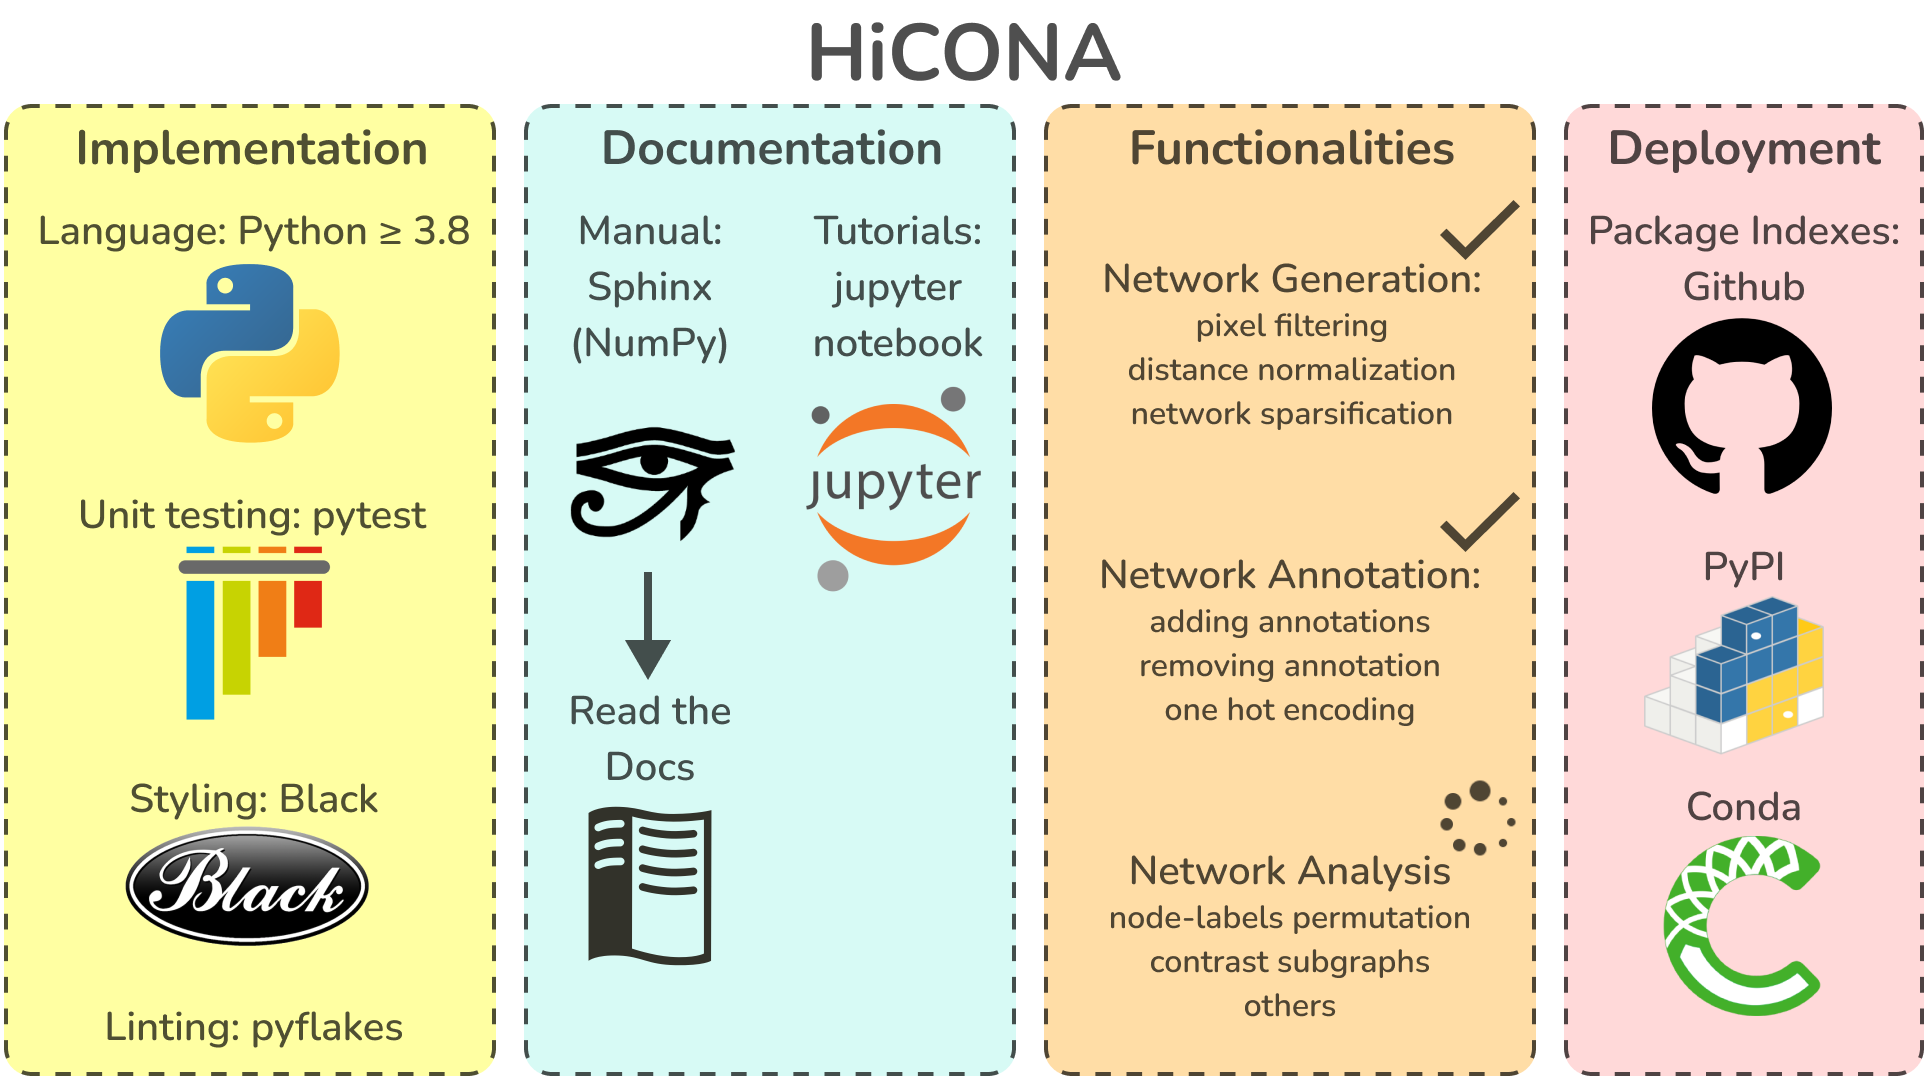
\includegraphics[width=1\textwidth]{roadmap.png}
  \caption{\textbf{Current state and future of HiCONA}. Main aspects regarding implementation, documentation, deployment and functionalities of HiCONA. Package documentation and deployment are still being worked on, though they are the next major step in the package development.}
  \label{fig:roadmap}
\end{figure}
